\chapter{$\gamma$-Astronomie} 
\label{ch:gamma}
Die Astronomie beschäftigt sich als Teilgebiet der Physik mit dem Universum, der Bewegung und Eigenschaften von Himmelskörpern wie Planeten oder Galaxien, interstellarer Materie und Strahlung. Betrachtete man früher nur Licht im optisch sichtbaren Bereich, so sind im 20. Jahrhundert einige zusätzliche Quellen dazugekommmen. Dazu zählen die von Viktor Hess durch Ballonversuche entdeckte kosmische Strahlung, die Röntgen- bzw. Gammastrahlung sowie die Neutrinostrahlung. Im Gegensatz zur kosmischen Strahlung, die überwiegend aus Protonen besteht, hat ungeladene Photonen- und Neutrinostrahlung den Vorteil, dass diese nicht durch elektromagnetische Felder abgelenkt wird und somit die Quellen dieser Strahlung leichter bestimmt werden können. Photonen haben zusätzlich den Vorteil, dass sie im Gegensatz zu Neutrinos, die nur schwach mit Materie wechselwirken, leichter zu detektieren sind. Ein interessantes Gebiet der letzten Jahre ist die VHE (Very High Energy)-Astronomie, die sich mit Quellen hoher Energie beschäftigt. Es gibt allerdings keine einheitliche Konvention einer Schwellenergie, die im Bereich zwischen $50 \unit{GeV}$ \cite{TeVCat2} und $100 \unit{GeV}$ \cite{DesignConcept} liegt. Das besondere an dieser Strahlung ist, dass sie so hochenergetisch ist, dass sie nicht mehr thermischen Ursprungs sein kann, sondern andere Erzeugungsmechanismen zugrunde liegen müssen.

\section{Entstehung hochenergetischer Strahlung}
\begin{description}
\item[Inverser Comptoneffekt]\hfill \\
Durch den Comptoneffekt können hochenergetische Photonen einen Teil ihres Impulses und ihrer Energie an ein freies Elektron übergeben. Dieser Prozess kann auch invers ablaufen und somit kann ein niederenergetisches Photon, zum Beispiel aus dem kosmischen Mikrowellenhintergrund ($E=250\unit{\mu eV}$ \cite{Grupen}), durch Interaktion mit einem hochenergetischem Teilchen eine Energie im Bereich der Gammastrahlung bekommen.
\item[Brems- und Synchrotonstrahlung]\hfill \\
Durchfliegen Elektronen starke Magnetfelder, wie es sie beispielsweise in der Nähe Neutronensternen gibt, oder starke elektrische Felder in der Nähe von Atomkernen, so erfahren sie eine Beschleunigung. Durch diese Beschleunigung werden Photonen abgestrahlt, deren Energie mit der Energie des Elektrons zunimmt.
\item[Zerfälle und Annihilation]\hfill \\ 
Hochenergetische Photonen können auch durch Zerfälle massiver Teilchen entstehen, wobei die Ruhemasse des Teilchens in kinetische Energie der Photonen umgewandelt wird. So zerfällt das neutrale Pion zum Beispiel zu 98,8\%  in zwei Photonen und setzt dabei eine Ruhemasse von $E_0=135\unit{MeV}$ \cite{PDG} um. Eine weitere Möglichkeit ist die Annihilation von Materie und Antimaterie. Auch hier wird die Ruheenergie der Teilchen in kinetische Energie umgewandelt. So entstehen bei der Elektron-Positron-Annihilation in Ruhe zwei Photonen mit der Energie $E=511\unit{keV}$.
%Diese Energien liegen allerdings noch weit unter der Grenze der VHE-Astronomie.
\end{description}

\section{Quellen hochenergetischer Strahlung}
Ziel der VHE-Astronomie ist es die Quellen hochenergetischer Gammastrahlung zu erforschen. Bild \ref{img:tevcat} zeigt alle bisher detektierten Gammaquellen.
\begin{description}
\item[Supernova Überreste]\hfill \\
Supernovae sind Explosionen von Sternen, die auf zwei Arten stattfinden können:\\Supernovae vom Typ Ia finden in Systemen von weißen Zwergen und Sternen statt. Ein weißer Zwerg ist ein ausgebrannter Stern, der größtenteils aus Sauerstoff und Kohlenstoff besteht. Saugt dieser weiße Zwerg Materie von einem anderen Stern ab, nimmt die Masse zu bis sie die Chandrasekhar-Grenze von ungefähr $1,4$ Sonnenmassen \cite{Grupen} überschreitet und durch den gestiegenen Gravitationsdruck die Kernfusion wieder startet.\\Kernkollaps-Supernovae entstehen aus Sternen. Nachdem diese ihren Wasserstoff- und Heliumvorrat verbrannt haben, folgt eine Gravitationskontraktion, die zu einer schnelle Abfolge von Kernfusionen schwererer Elemente führt. Nach dem Erreichen des stabilsten Elements ($\isotope[56]{Fe}$) kollabiert der Stern.\\Durch eine Supernova entsteht ein massives Objekt, das mit der durch die Explosion verteilten Materie interagieren kann.
\item[Pulsare]\hfill \\
Kollabieren die Überreste einer Supernova mit einem Durchmesser vonca. $10^6\unit{km}$ auf einen ca. $20\unit{km}$ großen,so entsteht ein Neutronenstern, der sich aufgrund der Drehimpulserhaltung sehr schnell dreht. Bleibt der magnetische Fluss durch die Oberfläche erhalten, entstehen große Magnetfelder ($\mathcal{O}(10^8\unit{T})$\cite{Grupen}). Sind Drehimpuls und Magnetfeld nicht parallel zueinander, so nennt man das entstandene Konstrukt Pulsar. In seinem rotierenden Magnetfeld können geladene Teilchen der interstellaren Materie beschleunigt werden, die somit Photonen abstrahlen.
\item[Schwarze Löcher und aktive galaktische Kerne]\hfill \\
Schwarze Löcher sind Objekte mit einer Gravitationskraft, die so stark ist, dass auch Photonen, die sich hinter dem Ereignishorizont befinden, nicht entkommen können. Durch die starke Anziehung entsteht eine Akkretionsscheibe in der große elektromagnetische Felder herrschen, durch die wiederum hochenergetische Photonen entstehen können.
Gerade in Zentren von Galaxien herrscht eine hohe Sterndichte, die dazu führt, dass hier supermassenreiche schwarze Löcher entstehen können. Diese können mit den großen Mengen an Plasma interagieren und strahlen häufig so hell, dass sie das Zentrum oder sogar den Rest der Galaxie überstrahlen können. Solche Quellen nennt man aktive galaktische Kerne (AGNs).
\item[Gamma Ray Bursts]\hfill \\
Gamma Ray Bursts (GRBs) sind kurzzeitige Strahlungsausbrüche mit einer typischen Länge von $10\unit{ms}$ bis $1000\unit{s}$, wobei Photonen eine Energie der Größenordnung von $10^{20}\unit{eV}$ \cite{tevstat} erreichen können. %cite
Die meisten GRBs lassen sich in kurzzeitige mit einer mittleren Dauer von 0,3s und langzeitige mit einer typischen Dauer von ungefähr 30s einteilen. Hinter den kurzzeitigen vermutet man Ereignisse mit kompakten Objekten, wie das Verschmelzen zweier Neutronensterne oder eines mit einem schwarzen Loch. Für die langzeitigen GRBs könnten Kernkollaps-Supernovae verantwortlich sein.
\item[Dunkle Materie]\hfill \\
Betrachtet man die Rotation von Galaxien, so stellt man fest, dass sich diese nicht durch sichtbare Materie erklären lassen. Um dieses Problem zu lösen, postuliert man die Existenz einer uns nicht bekannten Materieform, der dunklen Materie. Durch die VHE-Astronomie versucht man Erkenntnisse über diese zu gewinnen. Man sucht beispielsweise nach monoenergetischen Energielinien, die durch Selbstannihilation von dunkler Materie entstehen könnten.
\end{description}

\begin{figure}[htbp]
\centering
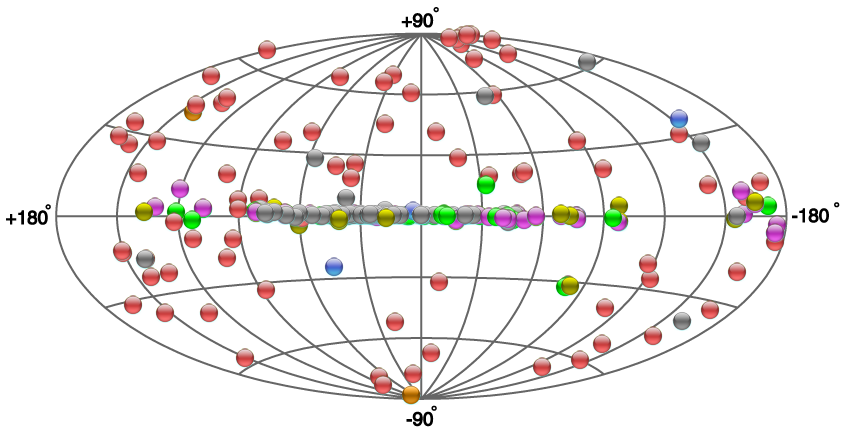
\includegraphics[width=\textwidth]{Images/tevcat.png}
\caption{Zu sehen sind alle von TeVCat registrierten und kategorisierten VHE-Quellen (ab einer Energie von $E~>50\unit{GeV}$\cite{TeVCat2}). Die roten Punkte stehen beispielsweise für AGNs, die violetten für PWNs und die grauen für unbekannte und unidentifizierte Quellen. \cite{TevCat}}
\label{img:tevcat}
\end{figure}


\section{Detektion von Strahlung}
Prinzipiell lässt sich zwischen bodengestützter und satellitengestützter $\gamma$-Astronomie unterscheiden. Durch den Einsatz von Satelliten vermeidet man den störenden Einfluss der Erdatmosphäre, muss dafür allerdings Abstriche in der Größe der Detektoren machen und mit hohen Kosten kalkulieren. Hier soll sich nur mit der günstigeren bodengestützten Variante beschäftigt werden. Dazu verwendet man sogenannte IACTs (Imaging Atmospheric Cherenkov Telescopes), die die Strahlung nur indirekt detektieren. Bild \ref{img:detection} zeigt die einzelnen Schritte der Detektion.

\subsection{Luftschauer}
Die Atmosphäre ist nur für Licht im optischen Bereich und Radiowellen durchsichtig. Treten hochenergetische Photonen in die Atmosphäre ein, findet Paarbildung statt. Das entstehende Elektron bzw Positron ist ebenfalls hochenergetisch und verliert hauptsächlich durch Bremstrahlung Energie, worauf die entstehenden Photonen wieder durch Paarbildung wechselwirken können. Hierdurch nimmt die Anzahl der Teilchen exponentiell zu, womit die durchschnittliche Energie pro Teilchen exponentiell abnimmt.
Ein Luftschauer der von einem 1TeV-Photon erzeugt wird, erreicht seine maximale Ausdehnung in einer Höhe von $8\unit{km}$ \cite{GB-VHE}. Danach ist die Energie der meisten Teilchen so gering, dass sie nur noch ionisieren.
% Der Luftschauer endet in einer Höhe von ungefähr 10km \cite{iwas}, wenn die Teichen niederenergetisch sind und die restliche Energie über Ionisation verlieren.
%\begin{equation}
%E_n=\frac{E_0}{2^n}
%\end{equation}\\
Neben den oben beschriebenen elektromagnetischen Schauern existieren noch hadronische und myonische Schauer. Hadronische Schauer entstehen wenn hochenergetische Hadronen in die Atmosphäre eindringen. Durch die Wechselwirkung von Hadronen entstehen häufig neutrale Pionen, die wiederum in Photonen zerfallen, wodurch wiederum ein elekromagnetischer Schauer entsteht, der allderdings einen anderen Ursprung hat. %Entstehen Myonen in einem Schauer, so besteht das Problem, dass diese kaum Energie abgeben und bei hoher Geschwindigkeit den Erdboden erreichen. Somit gibt nur ein Teil des Schauers die Energie ab und die Messung weicht von der Realität ab.

\subsection{Tscherenkow-Strahlung}
Tscherenkow-Strahlung tritt auf, wenn die Geschwindigkeit geladener Teilchen die Lichtgeschwindigkeit des sie umgebenden Mediums übersteigt. Hierbei polarisiert das geladene Teilchen auf seiner Trajektorie einzelne Atome, die Licht sphärisch abstrahlen. Wäre das Teilchen langsamer als die Ausbreitungsgeschwindigkeit in diesem Medium, würden die Wellen destruktiv interferieren und man würde keine makroskopischen Effekte beobachten. Da sich das Teilchen allerdings schneller als das Licht bewegt, entsteht ein Kegel konstruktiver Interferenz, und ein Lichtblitz breitet sich kegelförmig mit dem Öffnungswinkel
\begin{equation}
\theta = \arccos\left(\frac{1}{\beta n}\right) \label{eq:cherenkow}
\end{equation}\\
aus, wie in Abb \ref{img:cherenkow} gezeigt. Für Luft (in Bodennähe) ergibt sich somit ein maximaler Öffnungswinkel von $1,4^{\circ}$\cite{Grupen}. Da allerdings die Dichte der Luft in der relevanten Höhe kleiner ist, ist auch der Brechungsindex näher an 1 und der Tscherenkow-Winkel beträgt noch ungefähr $\theta = 1^{\circ}$\cite{Grupen}.
\begin{figure}[htbp]
\centering
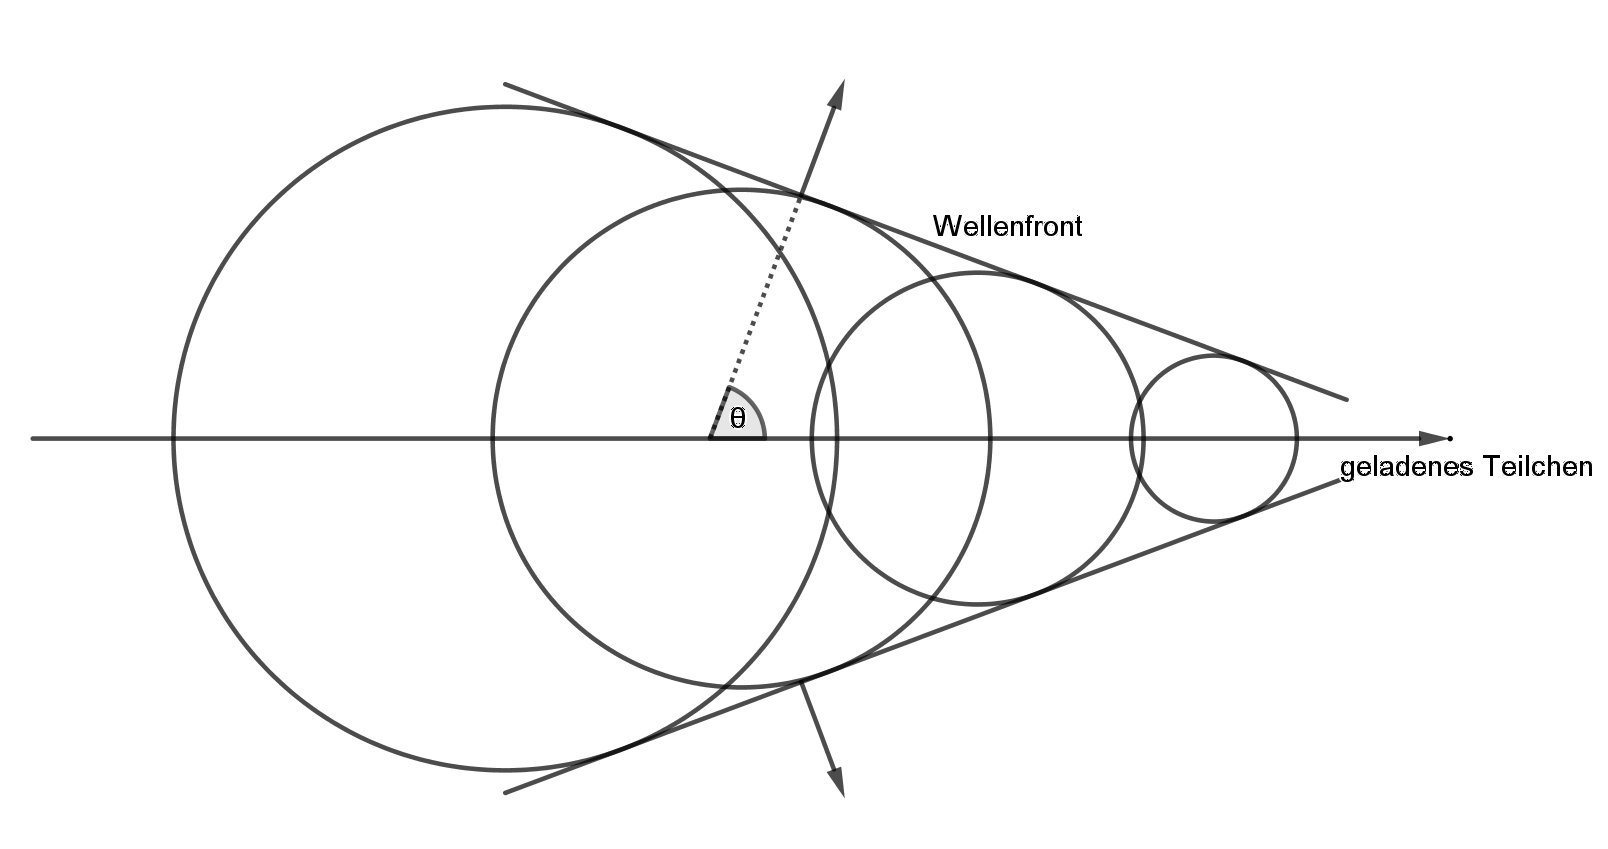
\includegraphics[width=0.7\textwidth]{Images/cherenkow.png}
\caption{Der Tscherenkow-Effekt: Ein geladenes Teilchen durchfliegt ein dielektrisches Medium mit einer Geschwindigkeit über der der Lichtgeschwindigkeit im Medium und erzeugt Wellenfronten.}
\label{img:cherenkow}
\end{figure}
Aus dem Winkel lässt sich die Geschwindigkeit des Teilchens rekonstruieren und bei bekannter Masse des Teilchens (in elektromagnetischen Schauern entstehen Elektronen als geladene Teilchen) auch der Impuls und die Energie.

\subsection{Bodengestützte Detektion der Tscherenkow-Strahlung}
Ziel der bodengestützten Variante ist es, das Tscherenkow-Licht der sekundären Teilchen aus dem elektromagnetischen Schauer zu detektieren. Bei einem Tscherenkow-Winkel von $\theta=1^{\circ}$ in $10\unit{km}$ Höhe und senkrechter Einstrahlung ergibt sich am Boden ein Lichtpool mit einem Durchmesser von $250\unit{m}$ \cite{DesignConcept}.% Somit müssen effektive Flächen in der Größenordnung von $10^4$ bis $10^5\unit{m^2}$ abgedeckt werden, um den gesamten Schauer zu detektieren. 
Typischerweise entstehen bei einem VHE-Photon $10^8$ bis $10^9$ Photonen, die innerhalb von wenigen Nanosekunden emitiert werden. Am Boden hat man somit typische Intensitäten von $10^3\unit{\frac{1}{m^2}}$.\\% die detektiert werden müssen.\\
Dazu verwendet man IACTs, die aus einem Reflektor und einem Detektor bestehen. Der Reflektor besteht aus einem oder häufig aus mehreren Spiegeln, die das Tscherenkow-Licht in der Brennebene bündeln. Bei großen Teleskopen muss der Reflektor parabolisch sein, bei kleineren wird darauf häufig aus Kostengründen verzichtet, da verschiedene Brennweiten für die Spiegel gebraucht werden.\\
Aufgrund der niedrigen Intensitäten und kurzen Zeitdauern der Tscherenkow-Blitze werden spezielle Kameras als Detektoren benötigt. Diese Tscherenkow-Kameras haben im Vergleich zu CCD-Kameras deutlich größere Pixel, so hat zum Beispiel die Kamera für einen Entwurf des SST \cite{gct} eine Pixelgröße von $6 \times 6\unit{mm^2}$ mit einer Zeitauflösung der Größenordnung $\mathcal{O}(1-10)\unit{ns}$. An jedem der Pixel ist zudem noch ein Photomultiplier angeschlossen, um das eingehende Signal zu verstärken. Aus den aufgenommenen Daten lässt sich mit Hilfe von Monte-Carlo-Simulationen die Richtung und die Energie des detektierten Photons rekonstruieren. 

\begin{figure}[htbp]
\centering
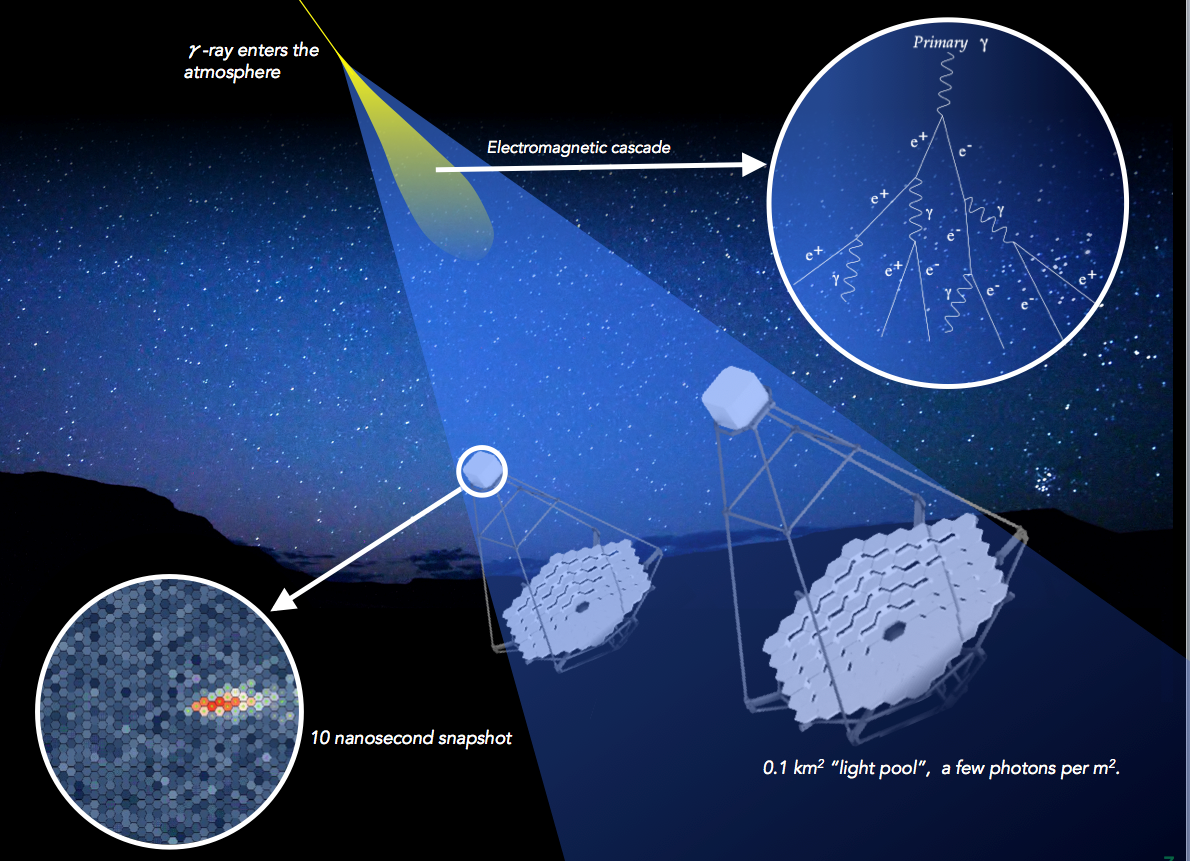
\includegraphics[width=\textwidth]{Images/detection.png}
\caption{Detektion hochenergetischer Strahlung: Das in die Atmosphäre eintretende Photon erzeugt einen elektromagnetischen Luftschauer (oben rechts), der wiederum Cherenkovlicht erzeugt, welches am Boden mit IACTs detektiert werden kann. Ein Detektionsbild ist unten links zu sehen.\cite{Flickr}}
\label{img:detection}
\end{figure}
